%Auswertung
\section{Wenner-Kartierung}

Die Wenner-Kartierung wurde auf einem 46\,m langen Profil E11-E12 senkrecht zum Basaltgang durchgeführt. Die Messprotokolle dazu befinden sich im Anhang in den Abbildungen  \ref{abb:Wenner1} und \ref{abb:Wenner2}. 
Die spezifischen Widerstände wurden bereits im Feld mit Hilfe der Formel~\eqref{eq:roh} aus Kapitel~\ref{sec:spezW} berechnet.
% In Tabelle \ref{tab:wenner} sind die gemessenen Werte des spezifischen Widerstands mit dem entsprechenden festgelegten Abstand zu sehen.
% Die spezifischen Widerstände wurden mit Hilfe der Formel \eqref{eq:roh} aus Kapitel \ref{sec:spezW} und den Werten der Tabellen \ref{abb:Wenner1} und \ref{abb:Wenner2} berechnet.
Die Abstände
der Messpunkte sind in der Mitte den Profils kleiner gewählt als außen, da wir dort den Basaltgang vermuten. Aus den Messergebnissen der Magnetik-Messungen konnte schon sehr genau abgeschätzt werden, wo der Basaltgang liegt.

%%%%%%%%%%%%%%%%%%%%%%%%%%%%%%%%%%%%%%%%%%%%%%%%%%%%%%%%%%%%%%%%%%%%
% \begin{table}[!ht]
% \centering
% \caption{Messwerte der Wenner-Kartierung}
% \begin{tabular}{ c  c  | c  c}
% \toprule
% Abstand in m  & Widerstand in $\Omega$m &  Abstand in m & Widerstand in $\Omega$m \\
% \midrule
% 0    & 15.873 & 25   & 32.673 \\
% 1    & 15.605 & 25.5 & 33.126 \\
% 2    & 16.036 & 26   & 29.951 \\
% 3    & 16.431 & 26.5 & 27.679 \\
% 4    & 16.658 & 27   & 25.546 \\
% 5    & 15.33  & 27.5 & 24.013 \\
% 6    & 15.155 & 28   & 23.626 \\
% 7    & 15.029 & 28.5 & 22.262 \\
% 8    & 15.044 & 29   & 21.232 \\
% 9    & 15.765 & 29.5 & 20.754 \\
% 10   & 18.122 & 30   & 20.354 \\
% 11   & 19.323 & 30.5 & 19.708 \\
% 12   & 20.27  & 31   & 21.024 \\
% 13   & 20.403 & 31.5 & 22.026 \\
% 14   & 20.054 & 32   & 22.442 \\
% 15   & 18.457 & 32.5 & 22.334 \\
% 15.5 & 18.217 & 33   & 21.789 \\
% 16   & 17.687 & 33.5 & 22.438 \\
% 16.5 & 17.456 & 34   & 22.927 \\
% 17   & 16.948 & 34.5 & 21.875 \\
% 17.5 & 16.859 & 35   & 20.88  \\
% 18   & 17.779 & 35.5 & 21.11  \\
% 18.5 & 18.37  & 36   & 20.109 \\
% 19   & 19.392 & 36.5 & 19.245 \\
% 19.5 & 20.363 & 37   & 19.105 \\
% 20   & 21.945 & 37.5 & 18.882 \\
% 20.5 & 23     & 38   & 18.774 \\
% 21   & 25.416 & 39   & 18.104 \\
% 21.5 & 30.071 & 40   & 18.712 \\
% 22   & 25.125 & 41   & 18.659 \\
% 22.5 & 31.057 & 42   & 19.165 \\
% 23   & 31.101 & 43   & 19.466 \\
% 23.5 & 32.759 & 44   & 20.332 \\
% 24   & 33.908 & 45   & 25.904 \\
% 24.5 & 33.561 & 46   & 20.623 \\
% \bottomrule
% \end{tabular}
% \label{tab:wenner}
% \end{table}
%%%%%%%%%%%%%%%%%%%%%%%%%%%%%%%%%%%%%%%%%%%%%%%%%%%%%%%%%%%%%%%%%%%%

In Abbildung \ref{abb:Wennerdiagr} sind die Messergebnisse
% aus Tabelle \ref{tab:wenner}
graphisch dargestellt. Wir gehen davon aus, dass der Basalt eine andere Leitfähigkeit hat als das Umgebungsmaterial und sich die magnetischen Eigenschaften und elektrische Leitfähigkeit 
gleichzeitig ändern. Das ist die Voraussetzung dafür, dass wir mit Hilfe unserer Ergebnisse aus der Magnetik unser Profil für die Geoelektrik festlegen können und in beiden Versuchen ähnliche Ergebnisse erhalten.

%%%%%%%%%%%%%%%%%%%%%%%%%%%%%%%%%%%%%%%%%
\begin{figure}[ht]
\centering
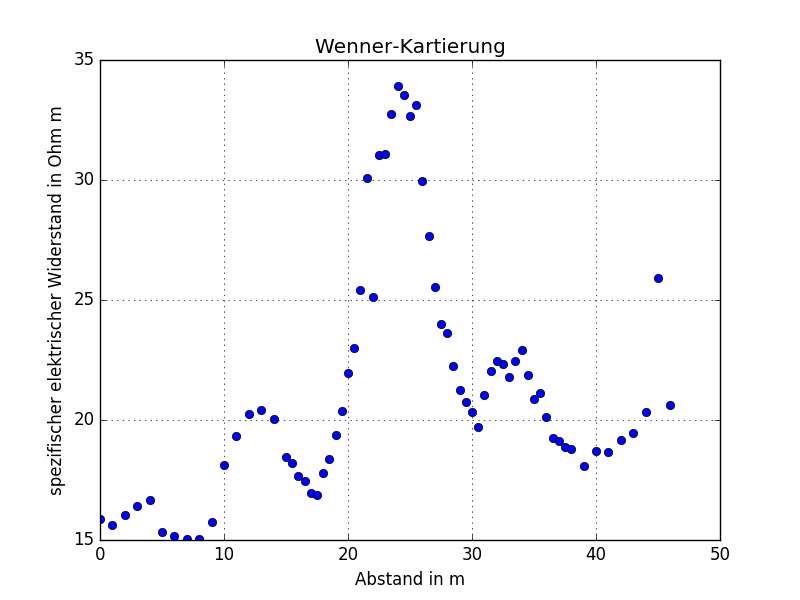
\includegraphics[width=0.8\textwidth]{fig/wennerkartierung.png}
\caption[Diagramm unserer Ergebnisse der Wenner-Kartierung]{Diagramm unserer Ergebnisse der Wenner-Kartierung. Der gemessene spezifische Widerstand ist gegen den Abstand zu unserem gewählten Null-Punkt aufgetragen. Der Null-Punkt wurde so gewählt, dass er mit dem Null-Punkt der Tomographie übereinstimmt}
\label{abb:Wennerdiagr}
\end{figure}
%%%%%%%%%%%%%%%%%%%%%%%%%%%%%%%%%%%%

Deutlich zu sehen ist ein Maximum des spezifischen Widerstands in der Mitte des Diagramms \ref{abb:Wennerdiagr}.
Dies weist darauf hin, dass der Basaltgang wie vermutet in der Mitte unseres Profils liegt.
Rechts und links des großen Maximums sind weitere kleinere Nebenmaxima zu erkennen. Da wir den Untergrund nicht genau kennen, können wir nicht mit Sicherheit sagen, um was es sich dabei handelt. Wir vermuten, dass der Basaltgang etwas verwittert 
ist, sich z.B. durch Wasser Risse im Gestein gebildet haben. Hat sich nun zwischen dem abgespalteten Basalt leitfähiges Material eingelagert, wird an diesen Stellen ein geringerer spezifischer Widerstand gemessen.
Da die Nebenmaxima nicht die gleiche Höhe haben wie das Maximum in der Mitte, ist es auch wahrscheinlich, dass der Basaltgang nicht nur durch Risse unterteilt ist. Wir gehen davon aus, dass der Basalt an den Rändern sehr stank verwittert ist.
Grob stimmen unsere Erkenntnisse mit denen der Magnetik überein.
%Grob genauer!!??? Was stimmt überein?

\section{Tomographie}

In Abbildung \ref{abb:Tomographie} sind die Ergebnisse der Tomographie-Messung zu sehen. Die obere Abbildung zeigt die von uns gemessenen Werte für den scheinbaren spezifischen Widerstand. Die Inversion der Werte, also ein Modell wie der Untergrund 
wirklich aussehen könnte, ist im unteren Diagramm zu sehen. In der Mitte ist dargestellt, welche Widerstandswerte man gemessen hätte, wenn der Untergrund dem berechneten Modell entsprechen würde.
Die beiden oberen Diagramme sind nahezu identisch, also sehr ähnlich. Das bedeutet dass, das berechnete Modell unsere gemessenen Werte sehr gut beschreibt.

%%%%%%%%%%%%%%%%%%%%%%%%%%%%%%%%%%%%
\begin{figure}[ht]
\centering
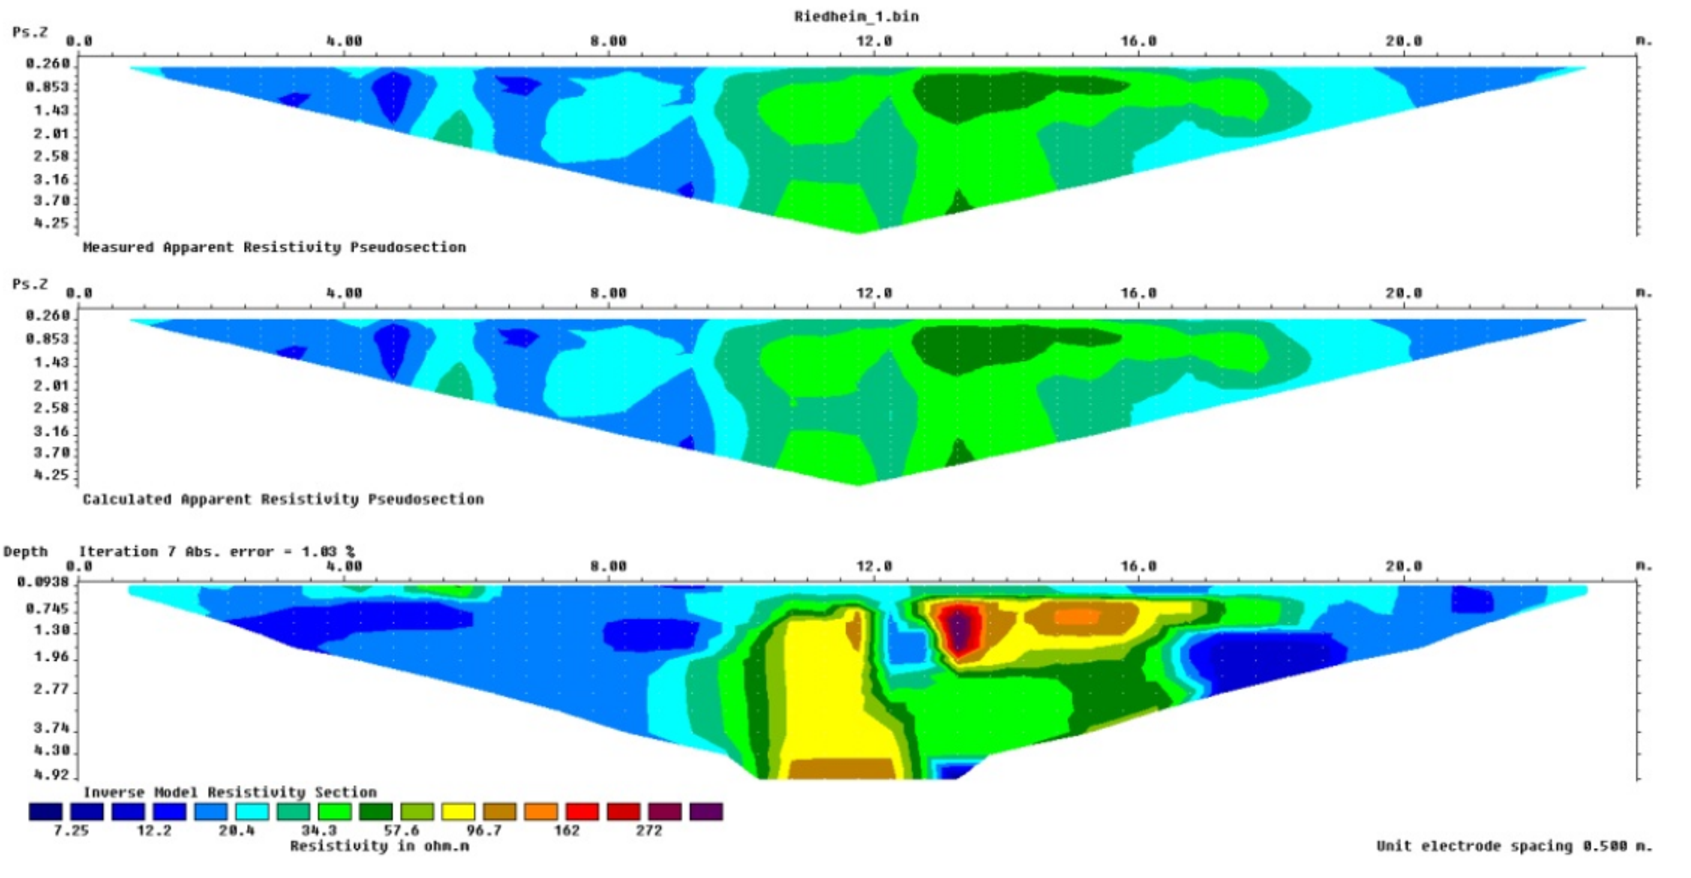
\includegraphics[width=\textwidth]{fig/Tomographie.pdf}
\caption[Tomographie-Modell]{Tomographie-Modell. Als Anfangspunkt der Messung wurde das obere Ende der Profillinie gewählt.}
\label{abb:Tomographie}
\end{figure}
%%%%%%%%%%%%%%%%%%%%%%%%%%%%%%%%%%%%

Bei dem Abstand 13\,m ist eine sehr starke Anomalie von ca. $ \SI{300}{\Omega m}$. Die Anomalie ist jedoch sehr klein und oberflächennah. Links davon ist eine zweite, sehr deutliche Anomalie zu sehen, die in dem gemessenen Bereich
mit zunehmender Tiefe größer wird. Der spezifische Widerstand ist hier aber nur maximal etwa $\SI{100}{\Omega m}$.
Etwa $\SI{2}{m}$ entfernt von der stärksten Anomalie, bei  $\SI{14}{m}$ beginnt eine dritte, oberflächennahe Anomalie.

Beim Vergleich mit den Ergebnissen der Wenner-Kartierung finden wir große Ähnlichkeiten. Die Tomographie deutet, ebenso wie die Wenner-Kartierung, darauf hin, dass der Basaltgang an der gemessenen Stelle grob in drei Teile unterteilt werden kann. Dies könnte von Karstverwitterung verursacht werden.

Allerdings sollte hier noch beachtet werden, dass die Wenner-Kartierung in einer Tiefe von $\SI{5}{m}$ vorgenommen wurde. Die Tomographie an ihrem tiefsten Punkt aber nur $\SI{5}{m}$ in die Tiefe geht. 

Zunächst wurde vermutet, dass die starke Anomalie dem globalen Maximum der Wenner-Kartierung entspricht. In der Tomographie sehen wir aber, dass die Differenz dieser stärksten Anomalie und den Nebenmaxima fast $\SI{200}{\Omega m}$ beträgt, was bei einer Skala von $\SI{0}{\Omega m}- \SI{300}{\Omega m}$ sehr viel ist. Wir haben vermutet, das diese Anomalie trotz der geringen Höhe die Tomographie beeinflusst.

Diese Annahme wurde überprüft, indem wir die Ortsangaben der beiden Diagramme verglichen haben. Leider passt die Wenner-Kartierung hier nicht mehr gut zur Tomographie. Vermutlich haben die Anomalien in den oberen Schichten wirklich kaum Einfluss auf die Wenner-Kartierung. Da wir diese in 5\,m Tiefe durchgeführt haben und das Tomographie-Modell eben hier aufhört, können wir die beiden Methoden eigentlich nicht vergleichen. Was aber auch ein interessantes Ergebnis ist, da wir nun sehen, dass die Messwerte der Wenner-Kartierung wirklich nahezu nur den spezifischen Widerstand in $\SI{5}{m}$ Tiefe wiedergeben.

\section{Sondierung}

Die Sondierung wurde auf dem Profil E21-E22 durchgeführt. Die Messwerte sind in Abbildung \ref{abb:Schlumberger1} und \ref{abb:Schlumberger2} im Anhang zu sehen. Aus ihnen werden mit Hilfe des Inversionsprogramms Ipi2win Modelle für die Schichten im Untergrund erstellt.
In Abbildung \ref{abb:Schlum1} und \ref{abb:Schlum2} sind die Ergebnisse zu sehen. Die schwarze Kurve ist die Fitkurve durch unsere Messpunkte und in blau ist das Modell des spezifische Widerstands des Untergrunds dargestellt. Die rote Kurve ist der scheinbare spezifische Widerstand, der sich aus diesem Modell ergibt.

\subsection{Modell mit drei Schichten}

Als erstes haben wir ein möglichst genaues Modell erstellt mit der Annahme, dass wir drei Schichten gegeben haben. Es müssen mindestens drei Schichten sein, da die schwarze Kurve in Abbildung \ref{abb:Schlum1} am linken Ende nach unten geht. Das Ergebnis ist in Abbildung \ref{abb:Schlum1} zu sehen. Der Fehler dieses Models lag bei unter 2\%. In Abbildung \ref{abb:SchlumTab1} ist die dazugehörige Tabelle mit dem berechneten spezifischen Widerstand $\rho$, der Dicke $h$ und Tiefe $d$ der jeweiligen Schichten.  Alle drei Werte nehmen mit der Tiefe zu, was sehr plausibel ist. Die erste Schichtgrenze ist in etwa $\SI{5}{cm}$ Tiefe und die zweite schon bei $\SI{43}{cm}$, die dritte erst bei etwa $\SI{8}{m}$. Diese Ergebnisse lassen sich leider nicht mit denen der Seismik vergleichen. 

%%%%%%%%%%%%%%%%%%%%%%%%%%%%%%%%%%%%
\begin{figure}[ht]
\centering
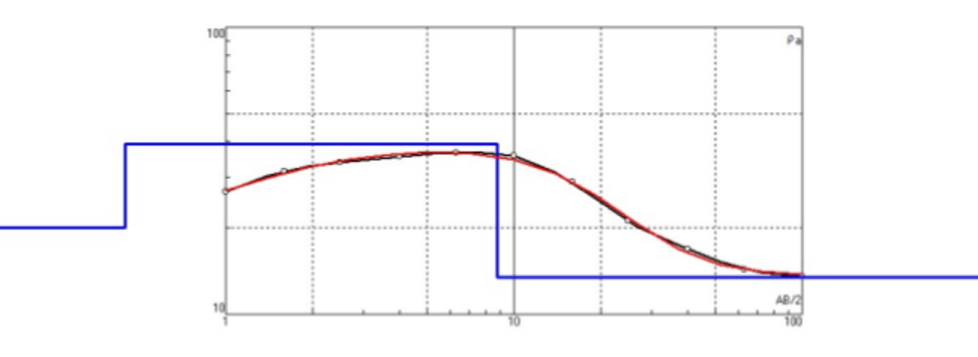
\includegraphics[width=0.8\textwidth]{fig/Schlumberger_3Schichten.pdf}
\caption{Inversionsmodel mit drei Schichten }
\label{abb:Schlum1}
\end{figure}
%%%%%%%%%%%%%%%%%%%%%%%%%%%%%%%%%%%%
%%%%%%%%%%%%%%%%%%%%%%%%%%%%%%%%%%%%
\begin{figure}[ht]
\centering
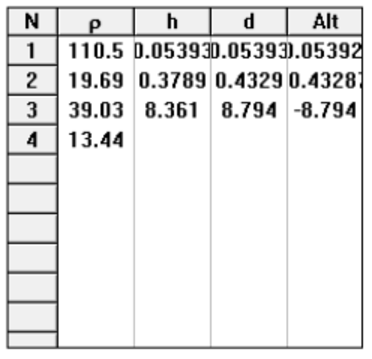
\includegraphics[width=0.3\textwidth]{fig/schlumbergerTabelle.pdf}
\caption[Daten zum Inversionsmodell mit drei Schichten]{Daten zum Inversionsmodell mit drei Schichten. $\rho$ bezeichnet den spezifischen Widerstand in $\Omega$m, $h$ die Schichtdicke in m, $d$ die Schichttiefe in~m}
\label{abb:SchlumTab1}
\end{figure}
%%%%%%%%%%%%%%%%%%%%%%%%%%%%%%%%%%%%

\subsection{Modell mir fünf Schichten}

Als zweites haben wir die Inversion ohne vorgegebene Maximalzahl der Schichten gemacht. Dabei wurde ein Modell mit 5 Schichten berechnet, welches in Abbildung \ref{abb:Schlum2} zu sehen ist. Die Tabelle mit den entsprechenden Werten ist in Abbildung \ref{abb:SchlumTab2} gegeben.

%%%%%%%%%%%%%%%%%%%%%%%%%%%%%%%%%%%%
\begin{figure}[ht]
\centering
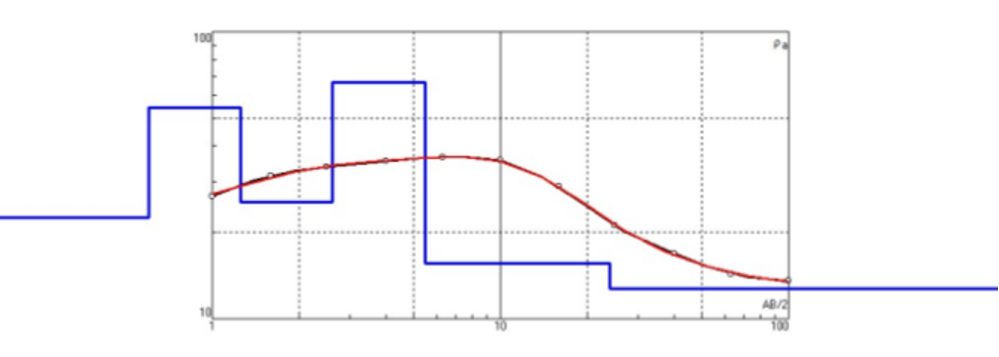
\includegraphics[width=0.8\textwidth]{fig/Schlumberger_5Schichten.pdf}
\caption{Inversionsmodell mit fünf Schichten}
\label{abb:Schlum2}
\end{figure}
%%%%%%%%%%%%%%%%%%%%%%%%%%%%%%%%%%%%
%%%%%%%%%%%%%%%%%%%%%%%%%%%%%%%%%%%%
\begin{figure}[ht]
\centering
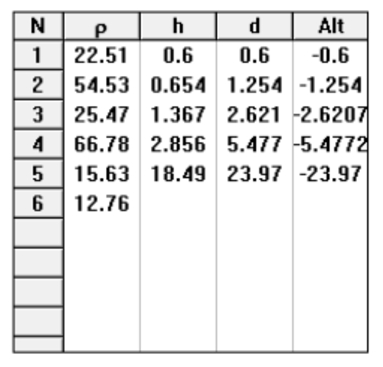
\includegraphics[width=0.3\textwidth]{fig/schlumbergerTabelle2.pdf}
\caption[Daten zum Inversionsmodell mit fünf Schichten]{Daten zum Inversionsmodell mit fünf Schichten. $\rho$ bezeichnet den spezifischen Widerstand in $\Omega$m, $h$ die Schichtdicke in m, $d$ die Schichttiefe in~m}
\label{abb:SchlumTab2}
\end{figure}
%%%%%%%%%%%%%%%%%%%%%%%%%%%%%%%%%%%%

Die erste Schichtgrenze liegt bei $\SI{60}{cm}$. Beim bohren mit Franz stießen wir in dieser Tiefe ebenfalls auf eine Schichtgrenze. Zu der reinen Erde an der Oberfläche kamen viele Kieselsteine dazu. Wenn wir davon ausgehen, dass sich damit auch die Leitfähigkeit des Untergrunds ändert, ist diese Schichtgrenze dieselbe und wir haben sie durch Bohrung nachgewiesen.

In $\SI{2,62}{m}$ Tiefe haben wir eine weitere Schichtgrenze. Interessanterweise haben wir in der Seismik in einer Tiefe von etwa $\SI{3,4}{m}$ ebenfalls eine Schichtgrenze gefunden. Die mit der Geoelektrik bestimmte Schichtgrenze liegt also noch im Fehlerbereich dieser Schichtgrenze. 
Gehen wir davon aus, dass sich hier die seismischen und geoelektrischen Eigenschaften des Untergrunds gleichzeitig ändern, haben wir mit dieser Messung das Ergebnis der Seismik-Messung bestätigt. 

Weitere Schichtgrenzen befinden sich in $\SI{1,3}{m}$, $\SI{5,5}{m}$ und $\SI{24}{m}$ Tiefe. Bei der 4. Schichtgrenze nimmt der spezifische Widerstand stark zu und bei der 5. Schichtgrenze sinkt sie auf einen niedrigeren Wert als den der ersten Schichten. Dies dann damit erklärt werden, dass hier der Grundwasserspiegel anfängt, wodurch die elektrische Leitfähigkeit erhöht wird.

Aus diesen Gründen nehmen wir an, das dieses Modell besser den tatsächlichen Gegebenheiten in Untergrund entspricht als das Modell mit nur drei Schichten.